\documentclass[addpoints,solutions]{exam}
\usepackage{multicol}
\usepackage{graphics,color,graphicx}
\usepackage{bm}
\usepackage[letterpaper, margin=1in]{geometry}
\usepackage{pgfplots}
\pgfplotsset{width=15cm, height=5cm,compat=1.9}
\newcommand{\ox}[1]{ \noindent\fbox{\parbox{\columnwidth}{#1 }}}
\newcommand{\e}{\epsilon_0}
\newcommand{\f}[2]{\frac{#1}{#2}}
\newcommand{\pderiv}[2]{\frac{\partial #1}{\partial #2}}
\newcommand{\bd}{\boldsymbol}

\begin{document}
\flushleft \textbf{Quiz: } (Topics 1.1 - 1.3) Rate of Change in Functions \hspace{2cm} Name: \rule{5cm}{0.1mm}
\noindent\hrulefill

\flushleft
\textbf{Directions: NO CALCULATORS.} Use the graph of the following function to answer the following:

\begin{figure}[htbp]
\begin{center}
\includegraphics[scale=0.25]{IMG_01}
\caption{Graph of $g$}
\label{default}
\end{center}
\end{figure}

\begin{questions}
\question The graph of a function $f$ is shown in the figure above for the interval $-6 \leq x \leq 6$. Use the graph of $f$ to answer the following.
\begin{multicols}{2}
\begin{parts}
\part On what open interval(s) is $f$ increasing?
\part On what interval(s) is $f$ decreasing?
\end{parts}
\end{multicols}
\end{questions}

\hrule
\vspace{1cm}
This is a test $\int_0^\infty f\left(x\right)$ \\
\vspace{1cm}
dfsfsf

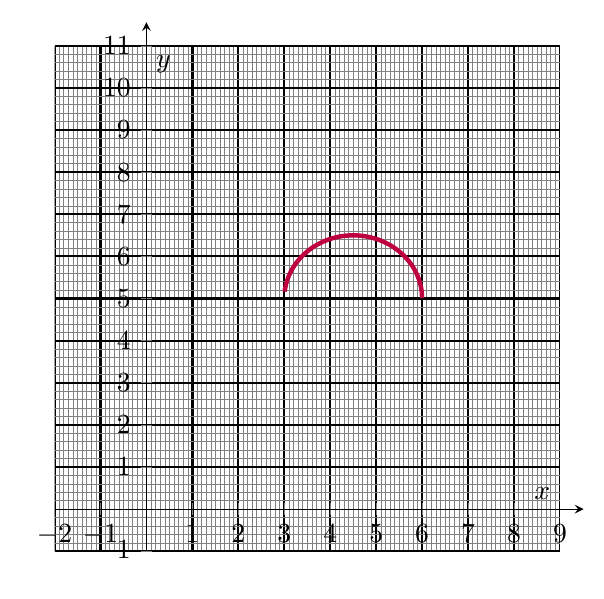
\begin{tikzpicture}
\begin{axis}[
  %axis lines = left,
  axis lines = middle,
  axis line style={-stealth,shorten >=-3mm},
  width=8cm,
  height=8cm,
  xlabel ={$x$},
  ylabel ={$y$}, 
  xmin=-2, xmax=9,
  ymin=-1, ymax=11,
  xtick={-2,-1,...,9},
  ytick={-1,0,...,11},
  xmajorgrids=true, ymajorgrids=true,
  minor grid style = {very thin, gray},
  major grid style={solid, thick, black},
  xminorgrids=true, yminorgrids=true, minor tick num = 1,
  %grid style = dashed,
  minor x tick num = 9,
  minor y tick num = 4,
  %minor tick style = {thin, gray},
  %major tick style = {thick, black},
  minor tick style={draw=none},
  xticklabel style={/pgf/number format/.cd, fixed relative, precision=4, /tikz/.cd},
  yticklabel style={/pgf/number format/.cd,fixed relative,precision=3}]
  %style="yticklabel style={
  %/pgf/number format/precision=5,
  %/pgf/number format/fixed}",
  %scaled y ticks=false]

%\addplot[color=red]{exp(x)};
%\addplot[color=blue, samples=100]{x^2};

\addplot[color=purple, domain=-3:6, samples=1000, style=ultra thick]{5+sqrt(1.5^2-(x-4.5)^2)};
\end{axis}
\end{tikzpicture}

\includegraphics{standalone}
\includegraphics{IMG_02}
\includegraphics{Passwwater}

\begin{multicols}{2}
\begin{figure}[h!]
  \centering
  \includegraphics{Passwwater}
  \caption{Graph of $p$}
\end{figure}

\begin{figure}[h!]
  \centering
  \includegraphics{Passwwater}
  \caption{Graph of $q$}
\end{figure}
\end{multicols}



\end{document}